\documentclass[]{book}

%These tell TeX which packages to use.
\usepackage{array,epsfig}
\usepackage{amsmath}
\usepackage{amsfonts}
\usepackage{amssymb}
\usepackage{amsxtra}
\usepackage{amsthm}
\usepackage{mathrsfs}
\usepackage{color}
\usepackage{cleveref}

%Here I define some theorem styles and shortcut commands for symbols I use often
\theoremstyle{definition}
\newtheorem{defn}{Definition}
\newtheorem{thm}{Theorem}
\newtheorem{cor}{Corollary}
\newtheorem*{rmk}{Remark}
\newtheorem{lem}{Lemma}
\newtheorem*{joke}{Joke}
\newtheorem{ex}{Example}
\newtheorem*{soln}{Solution}
\newtheorem{prop}{Proposition}

\newcommand{\lra}{\longrightarrow}
\newcommand{\ra}{\rightarrow}
\newcommand{\surj}{\twoheadrightarrow}
\newcommand{\graph}{\mathrm{graph}} \newcommand{\bb}[1]{\mathbb{#1}}
\newcommand{\Z}{\bb{Z}} \newcommand{\Q}{\bb{Q}} \newcommand{\R}{\bb{R}}
\newcommand{\C}{\bb{C}} \newcommand{\N}{\bb{N}} \newcommand{\M}{\mathbf{M}}
\newcommand{\m}{\mathbf{m}} \newcommand{\MM}{\mathscr{M}}
\newcommand{\HH}{\mathscr{H}}
\newcommand{\Om}{\Omega}
\newcommand{\Ho}{\in\HH(\Om)}
\newcommand{\bd}{\partial}
\newcommand{\del}{\partial}
\newcommand{\bardel}{\overline\partial}
\newcommand{\textdf}[1]{\textbf{\textsf{#1}}\index{#1}}
\newcommand{\img}{\mathrm{img}}
\newcommand{\ip}[2]{\left\langle{#1},{#2}\right\rangle}
\newcommand{\inter}[1]{\mathrm{int}{#1}}
\newcommand{\exter}[1]{\mathrm{ext}{#1}} \newcommand{\cl}[1]{\mathrm{cl}{#1}}
\newcommand{\ds}{\displaystyle}
\newcommand{\vol}{\mathrm{vol}} \newcommand{\cnt}{\mathrm{ct}}
\newcommand{\osc}{\mathrm{osc}} \newcommand{\LL}{\mathbf{L}}
\newcommand{\UU}{\mathbf{U}} \newcommand{\support}{\mathrm{support}}
\newcommand{\AND}{\;\wedge\;}
\newcommand{\OR}{\;\vee\;}
\newcommand{\Oset}{\varnothing}
\newcommand{\st}{\ni}
\newcommand{\wh}{\widehat}

\DeclareMathOperator*{\argmax}{arg\,max}
\DeclareMathOperator*{\argmin}{arg\,min}


%Pagination stuff.
\setlength{\topmargin}{-.3 in}
\setlength{\oddsidemargin}{0in}
\setlength{\evensidemargin}{0in}
\setlength{\textheight}{9.in}
\setlength{\textwidth}{6.5in}
\pagestyle{empty}



\begin{document}


\begin{center}
	{\Large Math 3220-1 \hspace{0.5cm} HW 1}\\
	\textbf{NAME}\\ %You should put your name here
	Due: DATE %You should write the date here.
\end{center}

\vspace{0.2 cm}


\subsection*{Exercises for Section 2}

\begin{enumerate}
	\item\label{k-classes} Suppose each of $K$-classes has an associated target
	$t_k$, which is a vector of all zeros, except a one in the $k$th position.
	Show that classifying to the largest element of $\hat{y}$ amounts to
	choosing the closest target, $\min_k\|t_k-\hat{y}\|$, if the elements of
	$\hat{y}$ sum to one.
	\begin{soln}
		\newcommand{\normone}[1]{\sum_{i\ne #1}|\hat{y}_i|+|1-\hat{y}_{#1}|} Let
		$k^*=\argmax_k \hat{y}_k$ and suppose that there is $k'\le k^*$ such
		that $\|t_{k'}-\hat{y}\| < \|t_{k^*}-\hat{y}\|$.
		\begin{itemize}
			\item $\ell_1$ norm. It holds that
			      $\|t_k-\hat{y}\|_1=\sum_i|t_{k,i}-\hat{y}_i|=\sum_{i\ne
					      k}|\hat{y}_i|+|1-\hat{y}_k|$. Hence, we get
			      \begin{equation}\label{2.1-inequality}
				      \normone{k'} < \normone{k^*}\Rightarrow |\hat{y}_{k^*}|-|1-\hat{y}_{k^*}|
				      < |\hat{y}_{k'}|-|1-\hat{y}_{k'}|.
			      \end{equation}
			      But the function $f(y)=|y|-|1-y|$ is increasing in $[0,1]$
			      hence~\Cref{2.1-inequality} implies that
			      $\hat{y}_{k^*}<\hat{y}_{k'}$, reaching a contradiction.
			\item $\ell_2$ norm. Similarly, we get that
			      $\hat{y}_{k^*}(1-\hat{y}_{k^*})<\hat{y}_{k'}(1-\hat{y}_{k'})$
			      and since the function $f(y)=y(1-y)$ is increasing in $[0,1]$,
			      we get that $\hat{y}_{k^*}<\hat{y}_{k'}$, reaching a
			      contradiction.
		\end{itemize}
	\end{soln}

	\item\label{exact-distribution} Show how to compute the Bayes decision
	boundary for the simulation example in Figure 2.5.
	\begin{soln}
		If we know the exact probability distribution $\Pr[G,X]$,
		$X\in\mathbb{R}^p$, $G\in \mathcal{G}=\{B,O\}$, then we can probably
		also derive $f(X)=\Pr[B|X]=\Pr[B,X]/\Pr[X]$, namely the probability that
		$X$ maps to blue in reality. This assume that we also know $\Pr[X]$
		which is not necessary. Of course, $\Pr[O|X]=1-\Pr[B|X]$. So now, all we
		have to do is to check for each $x\in\mathbb{R}^p$, whether $f(x)>1/2$.
		For the case where $x\in\mathbb{R}$, this is trivial. We simply solve
		the equation $f(x)=1/2$. This also hold in general. So the points (in
		$\mathbb{R}$), the line (in $\mathbb{R}^2$), and the $(p-1)$-dimensional
		hyperplane (in $\mathbb{R}^p$), is the solution to the equation
		$f(x)=\Pr[B|X]=1/2$. See Figure~\ref{fig:exercise2.2} for another
		example.

		\begin{figure}[h]
			\label{fig:exercise2.2}
			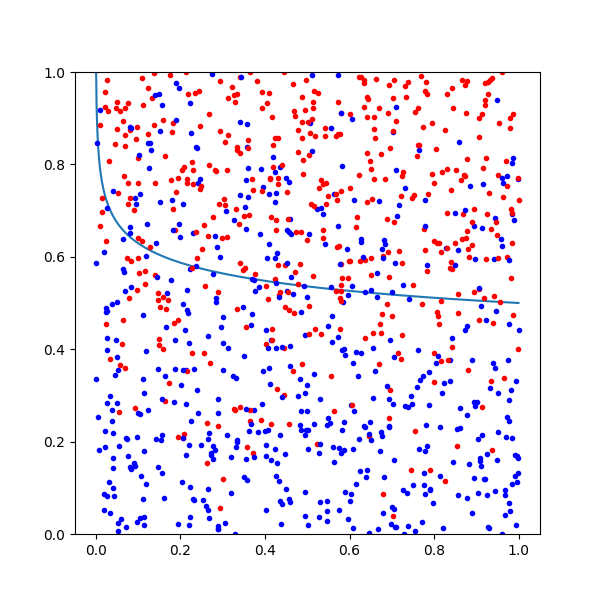
\includegraphics[width=8cm]{plots/ex22.png}
			\centering
			\caption{In this example we have computed the Bayes decision
			boundary when $X\sim U(0,1)^2$ and
			$\Pr[Y=\text{red}|X]=X_1^{1/10}X_2$. Therefore, the line is the
			solution to the equation $X_1^{1/10}X_2=1/2$.}
		\end{figure}
	\end{soln}

	\item\label{eq2.24} Derive equation 2.24. Consider $N$ data points uniformly
	sampled in a $p$-dimensional unit ball centered at the origin. Show that the
	median distance from the origin to the closest data point is given by the 
	expression $$d(p,N)=\left(1-\frac{1}{2}^{1/N}\right)^{1/p}.$$
	\begin{soln}
		We start with the cumulative distribution function (CDF) of the distance 
		of a random point from the origin. The volume of a $p$-dimensional ball of 
		radius $d$ is $V_p(d)=c_pd^p$, where $c_p$ is a value that does not depend
		on $d$. Therefore,
		\begin{equation}\tag{First trick to remember}
			F_D(d)=\Pr[D\le d]=\frac{V_p(d)}{V_p(1)}=d^p.
		\end{equation}
		Now it is useful to compute the CDF of the distance of the closest point
		$C=\min_{i\in[N]} D_i$. We have that 
		\begin{equation}
			\begin{split}
				F_C(d) &= \Pr[C\le d] \\
				&= 1-\Pr[C\ge d] \\
				&= 1-\Pr\left[\min_{i\in[N]} D_i \ge d\right] \\
				&= 1-\Pr[\forall i\in[N], D_i \ge d] \\
				&= 1-\prod_{i\in[N]}\Pr[D_i \ge d] \\
				&= 1-\Pr[D \ge d]^N \\
				&= 1-(1-\Pr[D \le d])^N \\
				&= 1-(1-d^p)^N.
			\end{split}
		\end{equation}
		By definition, the median $m$ is defined as $F_C(m)=1/2$. Hence, we get
		that $(1-m^p)^N=1/2$ and solving for $m$, we get
		\[m=\left(1-\frac{1}{2}^{1/N}\right)^{1/p}.\]
	\end{soln}

\end{enumerate}



\end{document}


